% @Author: Ren Qingjie
% @Date:   2017-05-28 23:06:23
% @Last Modified by:   Ren Qingjie
% @Last Modified time: 2017-05-30 16:40:30

% % \documentclass{article}
% \documentclass[xcolor=dvipsnames]{beamer}
% \usecolortheme[named=Maroon]{structure}
% \usetheme{Boadilla}
\documentclass{beamer}
\usecolortheme{UMONS}
% \usetheme{iut}
\usetheme{UMONS}
 \useoutertheme{UMONS}
\usepackage{helvet}
\title[FOF]{Fund of Funds}
\author{Qi Zhou, Wang Zhe, Ren Qingjie}
\institute{School of Physics \& School of Economics, Peking University}



\begin{document}
\maketitle



\begin{frame}
	\begin{itemize}
		\item{In this part, we would explore the relationship between the fund market and the retirement market.}
		\item{The Fund of Funds is favoured by risk averter, especially for those who have retired.}
		\item{There might be cointegration relationships bewteen the two markets.}
	\end{itemize}
	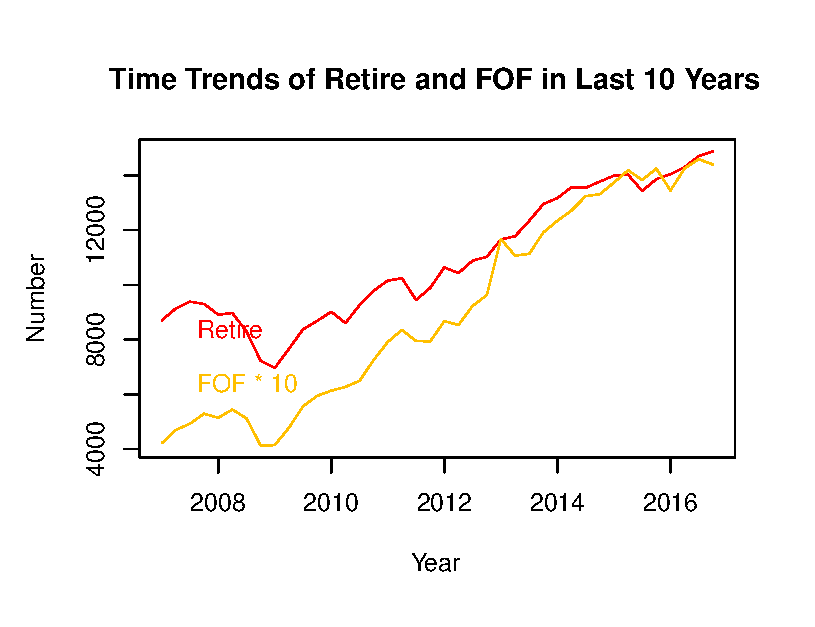
\includegraphics[scale=0.4]{3-0-1.eps}
	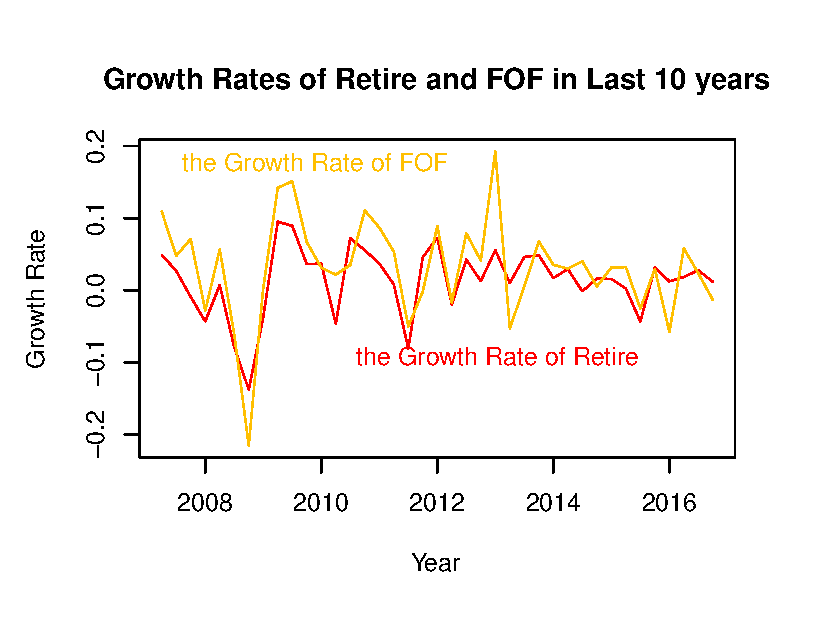
\includegraphics[scale=0.4]{3-0-2.eps}
\end{frame}


% 单位根检验 Unit Root Test
\begin{frame}{Unit Root Test}
	% \bigskip
	% 3 tests are employed here: \bold{ADF-Test}, \bold{KPSS-Test} , and \bold{PP-Test}
	3 tests are employed here: ADF-Test, KPSS-Test, and PP-Test (Phillips-Perron Test).

	Unit Root Test of Retire\\
	\par
	\begin{tabular}{|r |c |c |c| c|}
		\hline
		Test Method&Statistics & 10pct & 5pct & 1pct \\  \hline
		ADF & 1.64 &-1.61 & -1.95&-2.62 \\  \hline
		KPSS & 1.01 & 0.35 & 0.46 & 0.74 \\  \hline
		PP & 0.23 & *  &0.26 & *\\  \hline
	\end{tabular}
	\\
	\bigskip
	Unit Root Test of the Difference of Retire \\
	\begin{tabular}{|r |c |c |c| c|}
		\hline
		Test Method&Statistics & 10pct & 5pct & 1pct \\  \hline
		ADF & -2.31 &-1.61 & -1.95&-2.62 \\  \hline
		KPSS & 0.18 & 0.35 & 0.46 & 0.74 \\  \hline
		PP & 1.55 & *  &0.26 & *\\  \hline
	\end{tabular}	
	\\
	\bigskip
	\par
	Unit Root Test of FOF \\
	\begin{tabular}{|r |c |c |c| c|}
		\hline
		Test Method&Statistics & 10pct & 5pct & 1pct \\  \hline
		ADF & 2.53 &-1.61 & -1.95&-2.62 \\  \hline
		KPSS & 1.07 & 0.35 & 0.46 & 0.74 \\  \hline
		PP & -0.16 & *  &0.26 & *\\  \hline
	\end{tabular}
	\par
	Unit Root Test of difference of FOF \\
	\begin{tabular}{|r |c |c |c| c|}
		\hline
		Test Method&Statistics & 10pct & 5pct & 1pct \\  \hline
		ADF & -3.40 &-1.61 & -1.95&-2.62 \\  \hline
		KPSS & 0.11 & 0.35 & 0.46 & 0.74 \\  \hline
		PP & -40 & *  &0.26 & *\\  \hline
	\end{tabular}

\end{frame}
\begin{frame}{Unit Root Test}
	3 tests are employed here: ADF-Test, KPSS-Test, and PP-Test (Phillips-Perron Test). \\
	\begin{tabular}{|l| c| c| c|}
	\hline
	\textsc{Test} Method &  ADF   & KPSS &  PP   \\ \hline
	FOF 				 &  2.53  & 1.07 & -0.16 \\ \hline
	diff(FOF) 			 & -3.40  & 0.11 & 40 	 \\ \hline
	Retire 				 &  1.64  & 1.01 & 0.23  \\ \hline
	diff(Retire) 		 & -2.31  & 0.18 & 1.55  \\ \hline
	10pct 				 & -1.61  & 0.35 &   * 	 \\ \hline
	5pct 				 & -1.95  & 0.46 & 0.26  \\ \hline
	1pct 				 & -2.62  & 0.74 &   * \\ \hline

	\end{tabular}

\end{frame}


%  模型1, Model 1
\begin{frame}{Cointegration Relationship 1}
	First, estimate relationship between FOF and Retire.\\
	$FOF_t = \alpha + \beta * Retire_t + \mu_t$
	\begin{center}
	\begin{figure}
		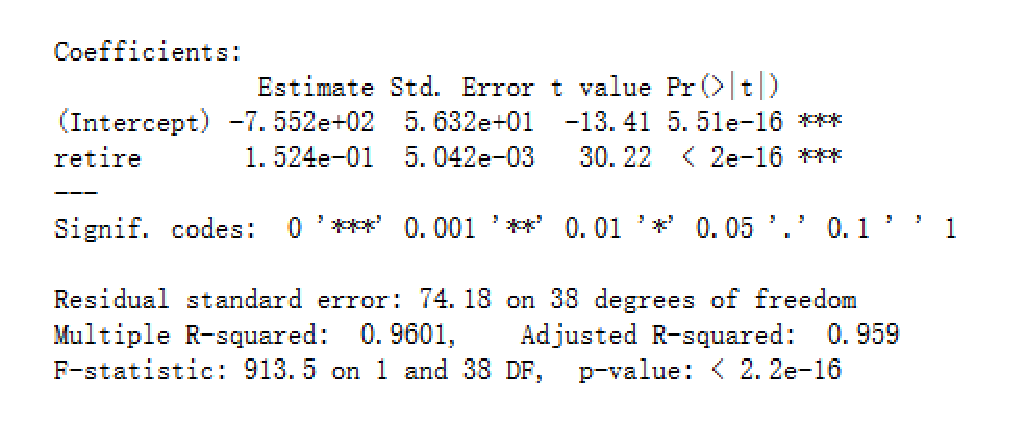
\includegraphics[scale=0.4]{3-3.eps}
	\end{figure}
	\end{center}

	Next, do unit root test on $\mu_t$. The results show that $\mu_t$ is white noise sequence. So two $I(1)$ processes combines to one $I(0)$ process. It indicates the cointegration relationship between FOF and Retire. And the cointegration vector is $(1, -0.15)$.
\end{frame}


\begin{frame}{Error Correction Model 1}
	Establish Error Correction Model use lags of FOF and Retire, and the residuals got before. Let $y = diff(FOF)$ and $x = diff(Retire)$ . And set the ecm equation as $y_t = \alpha_1 y_{t-1} + \alpha_2 y_{t-2} + \alpha_3 y_{t-3} + \alpha_4 y_{t-4} + \beta_0 x_t+\beta_1 x_{t-1} + \gamma r_{t-1} + \epsilon_t$.\\
	The results are as follows.
	\begin{center}
	\begin{figure}
		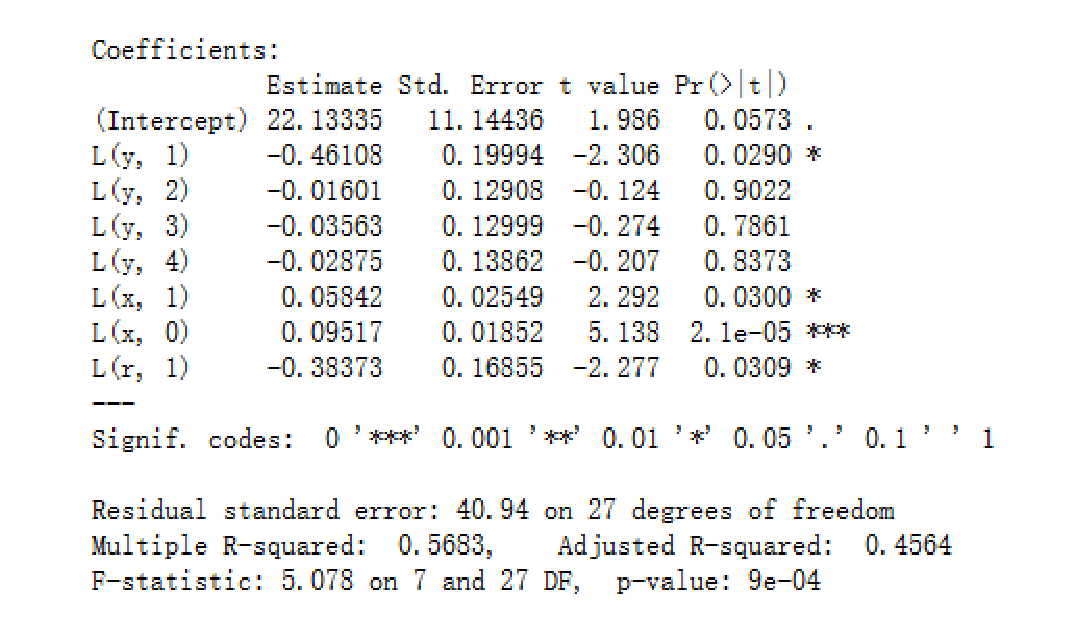
\includegraphics[scale = 0.5]{3-1-ecm.eps}
	\end{figure}
	\end{center}
\end{frame}


% 模型2, Model 2
\begin{frame}{Cointegration in Log}
	The $\log$ function is usually employed when dealing with macro-data. \\
	The Unit Root Test of $\log(FOF)$ and $\log(Retire)$ are as follows.
	
	\begin{tabular}{|l| c| c| c|}
	\hline
	\textsc{Test} Method &  ADF   & KPSS &  PP     \\ \hline
	log(FOF)			 &  2.28  & 1.07 & -1.04   \\ \hline
	diff(log(FOF)) 		 & -3.74  & 0.10 & -28.59  \\ \hline
	log(Retire) 		 &  1.39  & 1.00 & -0.41   \\ \hline
	diff(log(Retire))	 & -2.67  & 0.12 & -25.56  \\ \hline
	10pct 				 & -1.61  & 0.35 &   * 	   \\ \hline
	5pct 				 & -1.95  & 0.46 & 0.26    \\ \hline
	1pct 				 & -2.62  & 0.74 &   *     \\ \hline

	\end{tabular}
\end{frame}


\begin{frame}{Cointegration Relationship 2}
	Repeat the process before.
	\begin{figure}
		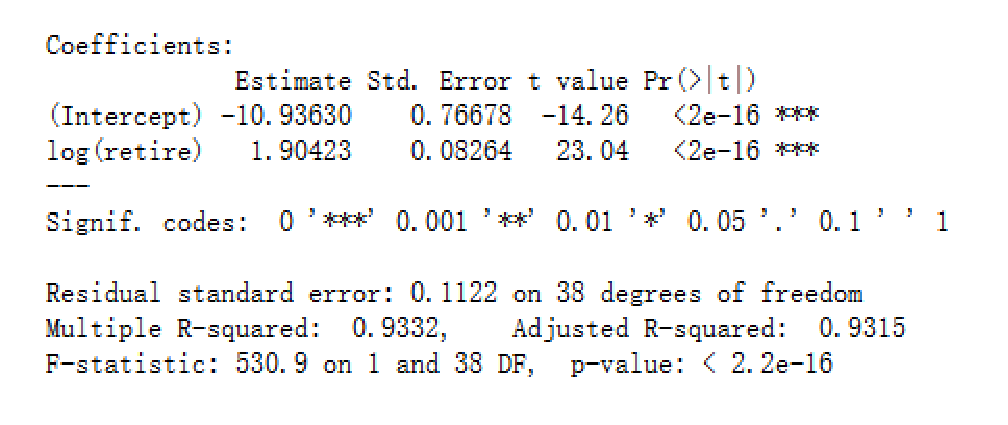
\includegraphics[scale = 0.4]{3-2-lm.eps}
	\end{figure}
\end{frame}


\begin{frame}{Error Correction Model 2}

	Let $y = diff(log(FOF))$ and $x = log(diff(Retire))$ 
	$y_t = \alpha_1 y_{t-1} + \alpha_2 y_{t-2} + \alpha_3 y_{t-3} + \alpha_4 y_{t-4} + \beta_0 x_t+\beta_1 x_{t-1} + \gamma r_{t-1} + \epsilon_t$.
	\begin{figure}
		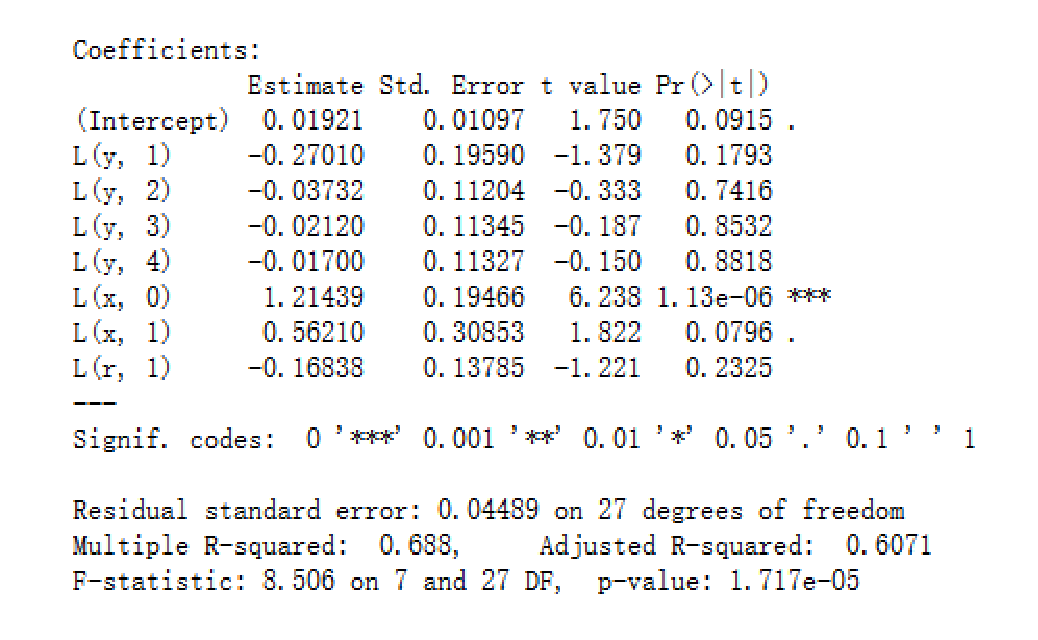
\includegraphics[scale = 0.4]{3-2-ecm.eps}
	\end{figure}
\end{frame}


% 模型3, Model 3
\begin{frame}{Cointegration Relationship Three}
\end{frame}


\begin{frame}{Error Correction Model Three}
\end{frame}


\end{document}
